% Chapter 1 - Introduction to Monsoon-Driven Crop Price Prediction
\chapter{Introduction to Monsoon-Driven Crop Price Prediction}
India's agri-economy is heavily dependent on the monsoon, which has a direct effect on the yield and market price of Kharif crops \cite{gadgil2006monsoon, sarkar2019monsoon}. The motivation for establishing a predictive system for crop prices based on seasonal rainfall patterns is introduced through this chapter. It sets the context and significance of the project, formulates the particular problem to be solved, and expresses the objectives of the work in clear terms. Also included is a description of the methodology adopted, the assumptions made in implementation, and the report structure that follows.
\section[Introduction]{\textbf{Introduction}}

Agriculture is the pillar of the Indian economy, with most of the population depending on cultivation for their livelihood \cite{birthal2015}. Of the various cropping seasons, the most important is the Kharif season, which depends very much on the monsoon \cite{gadgil2006monsoon}. Uncertainty of rainfall has direct bearing on crop production and, by extension, the market price of major commodities such as rice, maize, and pulses \cite{ray2019climate}. Volatility in price makes planning for cultivation and trading activities challenging for farmers as well as buyers \\cite{timmer2009price}.

To overcome this challenge, the project entitled \textit{Monsoon-Driven Crop Price Prediction} will predict the Kharif crop prices using past trends and local inputs. Utilizing government-sourced data and machine learning algorithms, the project aims to provide a trustworthy price forecasting tool in an interactive web environment. The system does not only forecast future prices but also presents past patterns of pricing visually, providing useful insights to inform decisions for farmers, traders, and policymakers \cite{jain2020deep, mahmud2025price}.

\begin{comment}
	You are allowed to use figures or diagrams which can help in introducing the topic acknowledging the source. For example, if you are introducing a particular topic, an appropriate figure can be used. The figure should be referenced in the text as Figure~\ref{fig:universe}.
	
	\begin{figure}[H]
		\centering
		
\includegraphics[scale=0.4]{Figures/universe}
		\caption{Sample picture of universe}
		\label{fig:universe}
	\end{figure}
\end{comment}

%These guidelines are provided to formally expose you to the various ethical %and technical issues involved in writing up your work and the format you are %required to adhere to while submitting your project report.
\section[Literature Review]{\textbf{Literature Review}}

This section reviews relevant academic contributions in the domain of crop price and yield prediction, with a focus on monsoon-related variability and regional forecasting models in India. The reviewed works span multiple methodologies including machine learning, deep learning, statistical modeling, and remote sensing. These papers collectively emphasize the importance of using climate data, particularly monsoon characteristics, in building reliable, region-specific price or yield prediction systems for agricultural decision-making.

\subsection{Impact of COVID-19 on Indian Agriculture \cite{cariappa2020impact}}
Cariappa et al. (2020) present a comprehensive assessment of the impact of the COVID-19 pandemic on Indian agriculture, highlighting how existing systemic problems were exacerbated by the crisis. The article delineates the implications of nationwide lockdowns on supply chain functioning, market access, and price stability. Specifically, farmers experienced huge hurdles in moving produce, accessing inputs, and securing buyers, resulting in enormous post-harvest losses and income volatility. The research specifically refers to the uneven incidence on smallholder farmers who were either devoid of digital platforms or storage facilities. The paper, based on state-wise case studies such as Karnataka, brings out stark variations in market recovery rates and resilience. The researchers propose the establishment of strong digital platforms to facilitate real-time access to market and weather data. This is closely aligned with our project's objectives, highlighting the importance of predictive mechanisms that not only curb monsoon-induced variability but also act as a shock absorber in the face of unprecedented disruptions. By providing a comprehensive overview of agricultural vulnerabilities under extreme scenarios, the research provides a robust contextual setting for our project.

\subsection{Price Forecasting with LSTM Networks \cite{mahmud2025price}}
Mahmud et al. (2025) offer an in-depth analysis of LSTM-based predictive models for use in the forecasting of agricultural commodity prices in India with a focus on their superiority in managing temporal relationships and nonlinearities in prices. The article considers various LSTM variants and compares them to traditional statistical models, including ARIMA and Holt-Winters, in the context of commodities like rice and pulses. One of the salient features of the study is the addition of external climatic variables such as rainfall, humidity, and temperature as input variables, which helped improve prediction quite noticeably. The authors verify their findings with multiple Indian state datasets, which helps ensure model robustness and applicability. Results indicate that models based on LSTM are consistently better than the conventional models, particularly when there is abrupt climatic fluctuation. The research ends by suggesting the inclusion of these models in decision support systems in real-time. For our Karnataka Kharif crops project, this paper is not just methodologically inspiring but also empirically justifying the inclusion of deep learning models based on climatic indicators. Stressing integration of temporal modeling with external variables reinforces the justification of our design decisions.

\subsection{Yield Forecasting Using ML in Karnataka \cite{kumar2024yield}}
Kumar et al. (2024) examine the use of machine learning models—namely Random Forest and Support Vector Regression (SVR)—for forecasting rice yield in Karnataka. Data come from government databases, with more than a decade of records on rainfall, humidity, temperature, soil type, and cropping patterns. By extensive training and calibration, Random Forest proved to be the most reliable and consistent model, exhibiting the capacity for identifying intricate nonlinear relationships among variables. The authors highlight the need for district-level models based on Karnataka's heterogeneous agro-climatic regions, citing that models aggregated at the state level tend to disregard local dynamics. Their research underscores the necessity of localized data and granular analysis, particularly in situations where variability at the regional level has the potential to heavily impact agriculture. Furthermore, the research offers a real-world framework for the application of environmental and soil information in predictive systems. Although the research is conducted using yield instead of price, the findings concerning spatial modeling, feature importance, and model scalability can be used directly in our project. This similarity serves to reinforce our focus on region-level forecasting and further validates our methodological emphasis.

\subsection{ARIMA-Based Forecasting of Agri Prices \cite{darekar2018price}}
Darekar and Reddy (2018) provide a systematic assessment of ARIMA models for agricultural commodity price forecasting using an intensive dataset from procurement centers of the government and wholesale markets. The commodities of interest are onions, rice, and wheat, and the analysis over a multi-year span is used to determine the robustness of the models during seasonal and economic cycles. They point out that ARIMA is good at capturing long-term trends and cyclical movements but falls short in capturing sudden changes due to unforeseen events such as policy changes, weather extremes, or supply shocks. The research recommends hybrid forecasting models that integrate the strengths of ARIMA with the flexibility of machine learning. Regarding model assessment, predictive accuracy is compared using metrics such as RMSE and MAPE, and the paper documents extensively preprocessing tasks like stationarity checks and parameter optimization. Although ARIMA provides a good benchmark, the research finds that dynamic learning-based models are better placed in unstable conditions such as India's agri-markets. This highlights our choice of including monsoon factors and machine learning models, utilizing ARIMA output as a baseline measure of performance for more complex models.

\subsection{Machine Learning in Crop Yield Forecasting \cite{ghetiya2024ml}}
Ghetiya et al. (2024) present a detailed description and empirical assessment of machine learning algorithms—namely, Decision Trees, Random Forest, and XGBoost—to forecast yields in Indian agriculture. The data cover 15 years and contain climate, soil characteristics, seed quality, and market inputs. The work experiments with various agro-climatic regions and indicates that the best predictive accuracy is achieved using XGBoost, especially with variable rainfall and fertilizer application. The authors present a strong argument for multi-source integration of data, referencing enhanced generalization and model stability. Of particular interest is their feature selection discussion, where agro-meteorological variables are always included as the most significant variables. Regional personalization is also highlighted as crucial, with the authors recommending that even within a state, model customization can pay substantial dividends. While it indirectly does not address price prediction, the understanding of feature significance and algorithmic prediction strengths gives our work a solid basis. The research reinstates our selection of ensemble models and supports the consideration we provide to regional data partitioning in our project.

\subsection{CNN-LSTM for Crop Price Prediction \cite{ragunath2025cnn}}
Ragunath and Rathipriya (2025) introduce a new deep learning model that integrates Convolutional Neural Networks (CNN) with Long Short-Term Memory (LSTM) networks in order to predict crop prices. The model is educated on an extensive dataset containing temporal price information, climatic data from regional areas, and spatial cropping patterns. The CNN module is employed to derive local features like district-level cropping intensity and market access, whereas the LSTM module detects temporal relationships and price trends over time. The hybrid model demonstrates considerable enhancement compared to individual CNN or LSTM models, yielding lower error rates in MAPE and RMSE measurements. The authors believe that the spatiotemporal combined modeling captures the multi-factorial aspect of agricultural prices better, especially in a monsoon-based state like Karnataka. Our research validates our philosophy of combining geographic and temporal factors to achieve a more solid and situation-aware prediction tool. More importantly, model interpretability and deployment in real-world scenarios make the paper a good reference for our prediction web interface implementation.

\subsection{Spatial Crop Suitability Mapping \cite{tripathi2021mapping}}
Tripathi et al. (2021) provide a spatial suitability analysis of Kharif crops in Karnataka based on Geographic Information System (GIS) methods coupled with machine learning classifiers. The article makes use of large environmental data sets such as rainfall, temperature, soil type, and historical cropping patterns to create suitability indices for various crops. The indices are utilized to identify best areas for individual crops, exposing ecological limitations and possibilities. A major takeaway is the relationship between ecologically suitability and market price instability—areas of lower suitability tend to have unstable prices with fluctuating yields. Although the study does not make explicit price forecasts, it offers a critical ecological benchmark that can be used to increase the explanatory value of any price forecasting model. The map outputs are additionally informative for policymakers and agricultural extension agents interested in the promotion of climate-resilient agriculture. By situating market results in the context of ecological viability, our paper fits squarely into our project's mission to provide region-specific crop price projections based on environmental information.

\subsection{Rainfall Variability in Karnataka \cite{henrich2020rainfall}}
Henrich et al. (2020) examine rainfall behavior in southern Karnataka for 60 years to identify long-term trends and unfolding anomalies. Based on India Meteorological Department data, the authors detect changes in the onset, length, and intensity of the monsoon season. Statistical methods include time series decomposition, anomaly detection, and spatial clustering, which show enhanced variability and delayed monsoon onset during recent decades. These results hold significant implications for agricultural planning and price predictions, as delayed rainfall influences sowing periods, production cycles, and thereby market supply. The paper urges adaptable agricultural methods and improved forecasting methods that can incorporate real-time weather reports. For our project, the applicability is in applying these rainfall patterns as predictive features to our machine learning algorithms. The research provides econometric evidence for the hypothesis that monsoon variability is a principal driver of crop price fluctuations in Karnataka.

\subsection{AI-Based Advisory Platform for Farmers \cite{singh2024ai}}
Singh and Sindhu (2024) detail the creation of an advisory system based on AI intended to support farmers' real-time decisions regarding crop selection, irrigation planning, and market price. The system brings together several data streams, such as weather patterns, soil conditions, and market prices, to offer individualized advice. Developed through ensemble machine learning methods and optimized for use in low-bandwidth settings, the software can be accessed through smartphones and feature phones. User studies of rural Haryana and Maharashtra districts reveal significant improvement in input optimization and yield performance. Although the system is not primarily designed for price prediction, its structure proves the utility and viability of consolidating disparate data feeds into one user interface. The focus on usability, accessibility, and regional customization provides essential lessons for our project's web app. It justifies the necessity for user-focused design and advocates the use of real-time, adaptive analytics within agricultural decision support systems.

\subsection{Deep Learning for Commodity Price Forecasting \cite{jain2020deep}}
Jain et al. (2020) perform an elaborate comparison of deep learning models for forecasting Indian daily commodity prices using LSTM, GRU, and BiLSTM models. The authors gather high-frequency prices from Agmarknet for rice, wheat, and pulses and find that BiLSTM consistently outperforms the other models in terms of several error measures owing to its capacity to learn both previous and subsequent contexts at training time. The paper further comprises an exhaustive discussion of data preprocessing methods such as normalization, handling outliers, and time-step optimization, all of which have a strong influence on model performance. The paper also focuses on deployment strategies, suggesting cloud-based options for scalability and real-time access. For our project, this paper provides a good grounding in neural architecture choice, hyperparameter choice, and deployment. It supports our choice of applying deep learning to time-series price prediction and gives practical advice on creating a strong and scalable prediction engine.

\section[Motivation]{\textbf{Motivation}}

Agriculture remains a key driver of Karnataka's economy, employing much of the rural labor force and generating a large percentage of the state's GDP \cite{niti2024, kgisac2023}. Yet, the production and prices of Kharif crops are extremely responsive to the arrival, spread, and intensity of the monsoon \cite{prasanna2014, gadgil2006monsoon}. Over the past few years, irregular patterns of rainfall have made it more challenging for farmers to predict crop production and market price \\cite{prasanna2014, reuters_mon2025}. It does not just impact their revenues but also goes on to influence sowing decisions, input procurements, and marketing strategies.

While Karnataka has been making strides in digital agriculture through several initiatives by the government, there remains an absence of localized data-driven solutions that can help farmers plan according to price trends \cite{niti2024_gov}. The majority of current solutions are either too generalized or unavailable to grassroots users. The project attempts to fill this void by specifically targeting Karnataka, leveraging its past crop prices and local conditions to develop a system that can forecast prices and display trends. The aim is to empower farmers with actionable data that mitigates reliance on middlemen and speculative pricing, which in turn helps in achieving improved financial returns and more resilient agricultural practices in the state.

\section[Problem Statement]{\textbf{Problem Statement}}

Kharif crop prices in Karnataka are highly seasonal and regional in nature, depending primarily on irregular monsoon trends and unstable market conditions \cite{prasanna2014, gadgil2006monsoon, henrich2020rainfall}. Farmers may not have access to prompt and accurate information on forthcoming price directions, and hence it becomes challenging for them to take well-informed decisions on crop choice, harvesting, and selling \cite{cariappa2020impact, jain2020deep}. This results in financial insecurity, exploitation by middlemen, and inefficient resource utilization \cite{singh2024ai, niti2024}. Even with the existence of historical data, there is no local, free platform today that uses this data to forecast crop prices in an easy-to-understand format \cite{tripathi2021mapping, mahmud2025price}. The issue solved by this project is the requirement for a predictive and graphical tool to estimate Kharif crop prices by providing time and location as inputs, assisting stakeholders in making enhanced decisions based on climatic and market conditions of Karnataka.

\section[Objectives]{\textbf{Objectives}}
The objectives of the project are:
\begin{enumerate}
	\item To gather, clean, and incorporate historical crop price and monsoon data for Karnataka from multiple government sources.
	\item To create a machine learning model that forecasts Kharif crop prices from temporal and geographic parameters.
	\item To create an interactive web page where a user can visualize historical trends and see future-predicted prices according to chosen time and location.
\end{enumerate}

\section[Brief Methodology of the project]{\textbf{Brief Methodology of the project}}

The entire project workflow is divided into several dependent stages: Data Processing, ML Engineering, Development, Deployment, and User Interaction. It starts with gathering and pre-processing data for Kharif crop prices and monsoon trends. The pre-processed data is utilized to train and test machine learning models in the ML Engineering Phase. After settling on an appropriate model, it is implemented in a web application in the Development Phase. The application is tested prior to deployment for use in production. End users are able to access the interface to get price forecasts and view past trends. A user interface feedback loop to model training enables future predictions to be improved.

\begin{figure}[H]
	\centering
	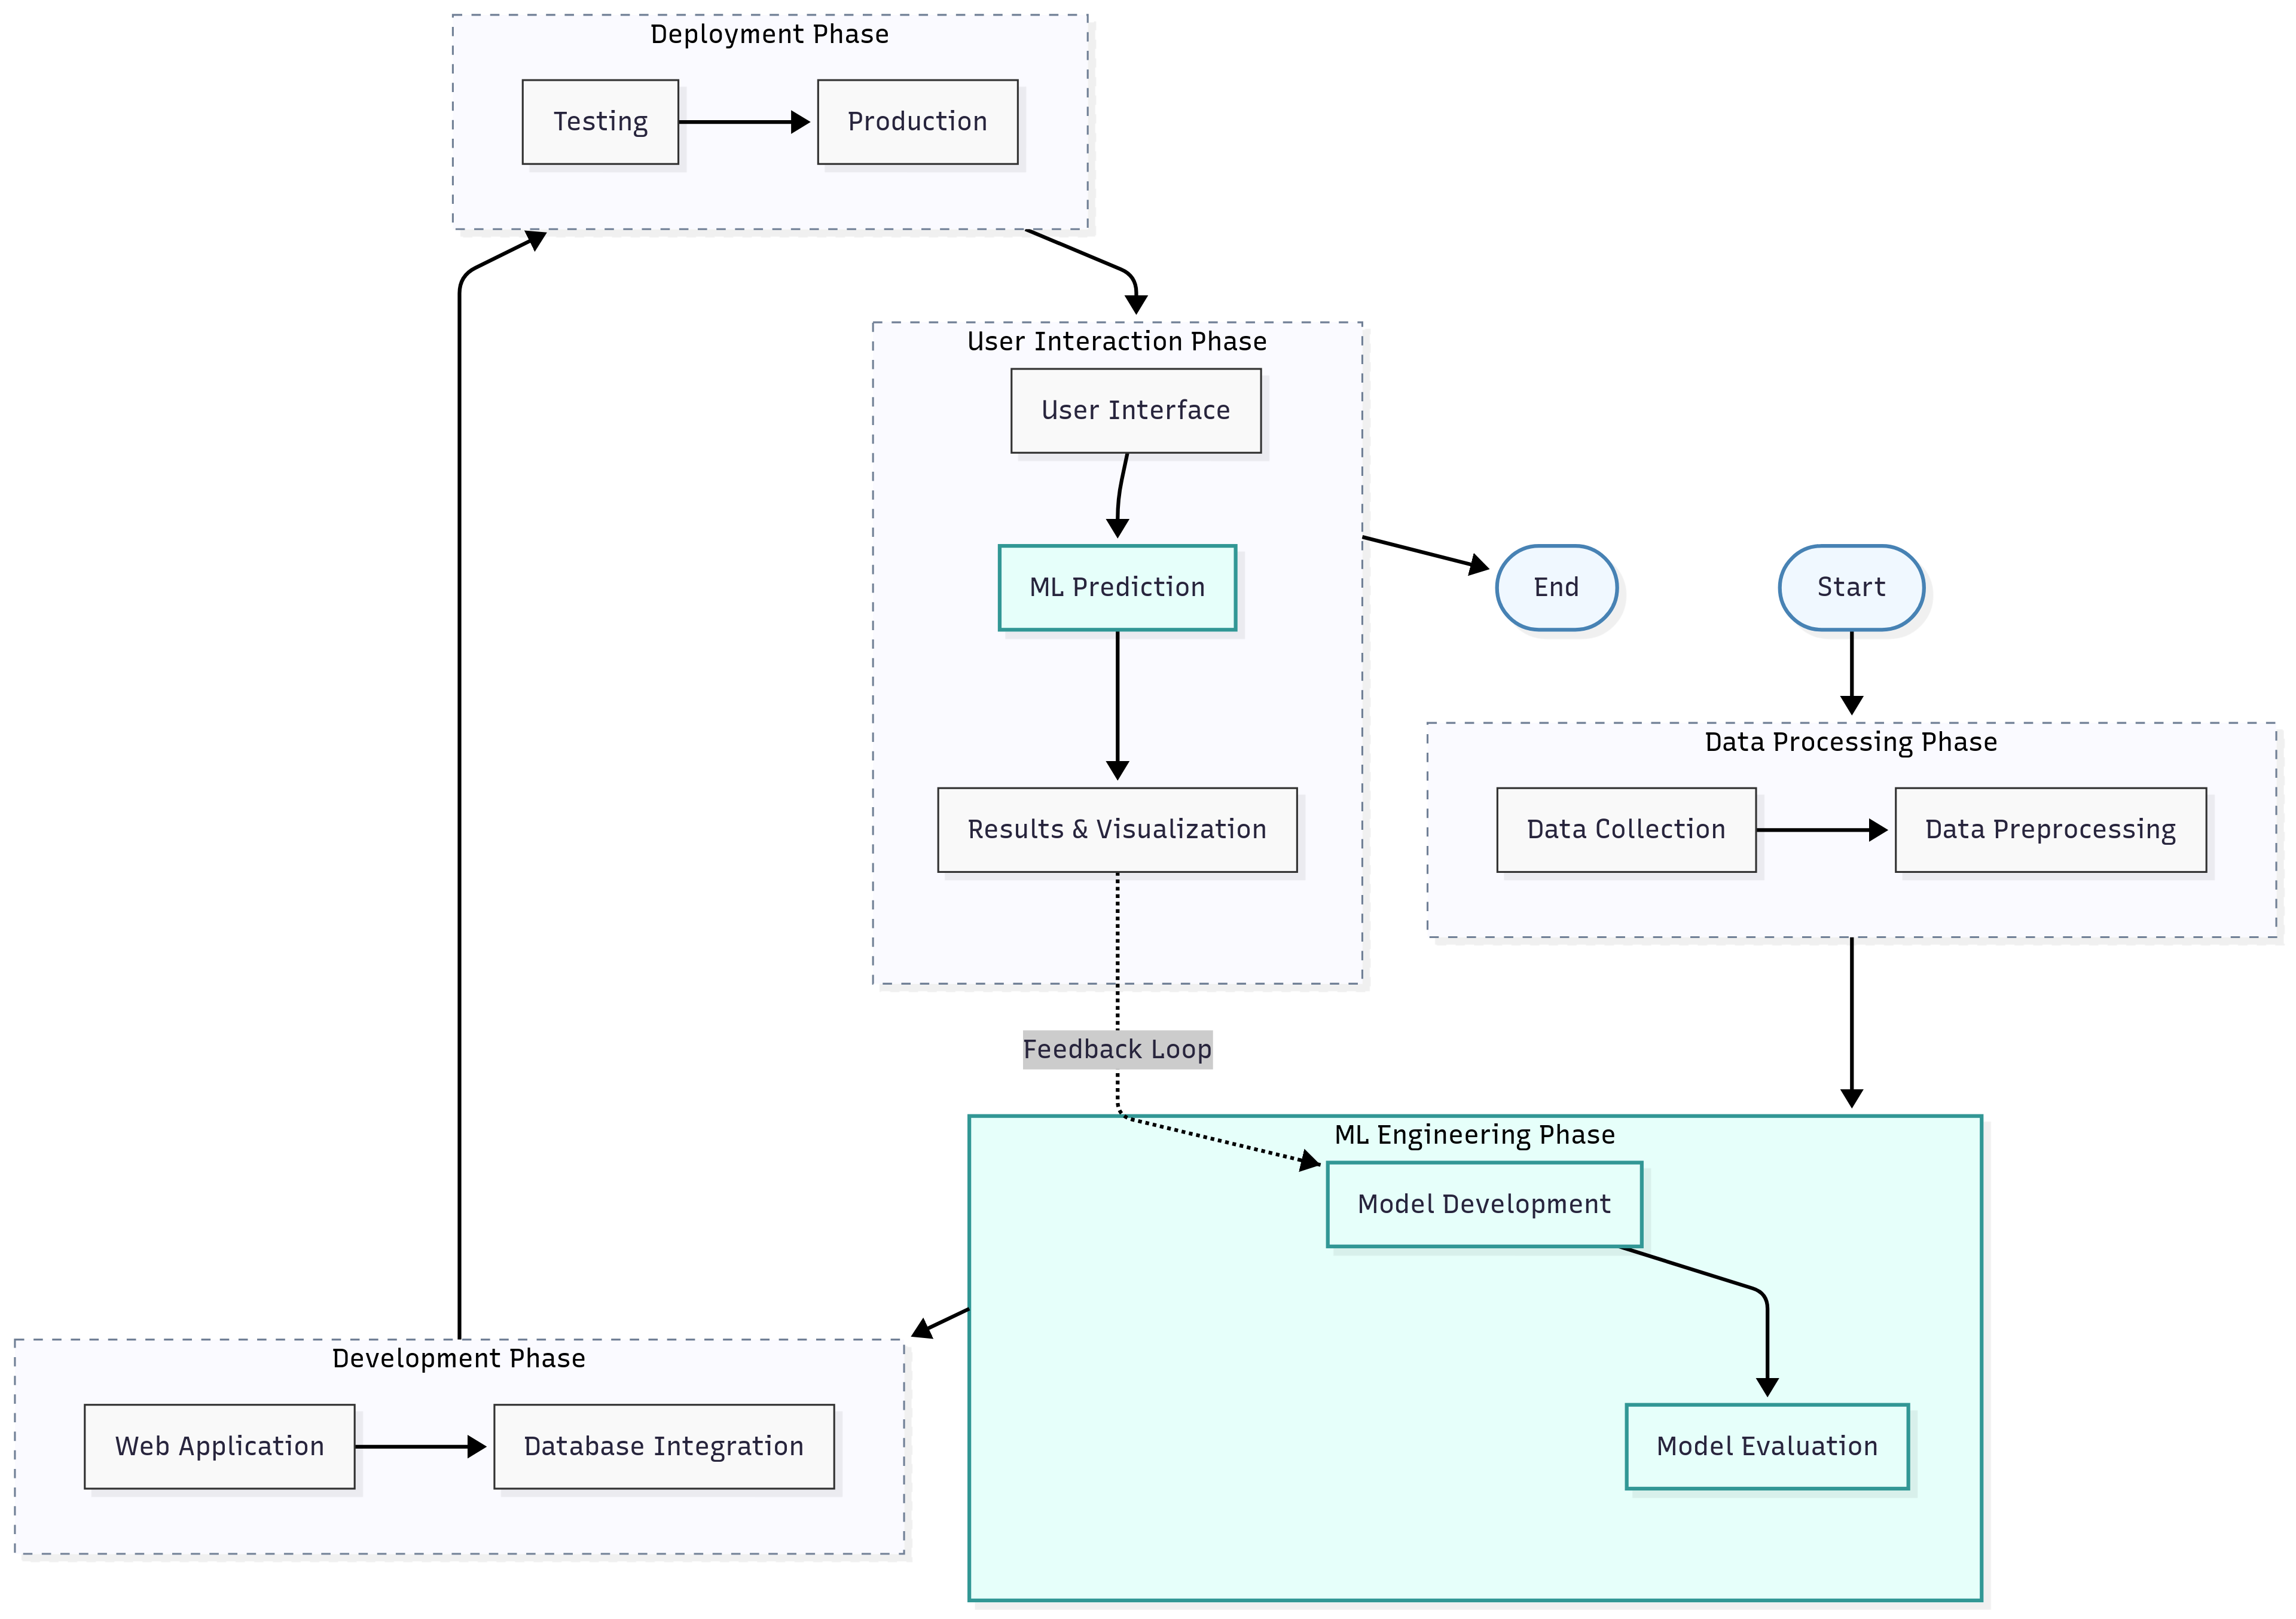
\includegraphics[width=0.95\textwidth]{Figures/Methodology_IDP.png}
	\caption{Overall Methodology of the Monsoon-Driven Crop Price Prediction System}
	\label{fig:methodology}
\end{figure}

\section[Assumptions made / Constraints of the project]{\textbf{Assumptions made / Constraints of the project}}

The following assumptions and constraints were considered during the development of the project:

\begin{itemize}
	\item It is presumed that the historical crop price data gathered from government sources are representative, reliable, and accurate of the market conditions prevailing in Karnataka.
	\item The model presumes that history of past prices and monsoon trends can be utilized as predictors of future prices with little interference from unforeseen external events like policy shocks, natural disasters, or random market surprises.
	\item It is assumed that the administrative limits and area classification employed in the dataset are constant over time for reasonable regional comparisons.
	\item One of the main limitations of the project is the limited availability and detail of historical data in some areas and crops, which can impact the accuracy of predictions in these regions.
	\item The project scope at present is restricted to the Karnataka state only and caters mostly to Kharif crops; expansion to other states or crop seasons would involve considerable restructuring of data and retraining the model.
	\item The model does not yet include non-climatic influences such as storage prices, movement costs, government subsidies, or market intervention that also affect crop prices.
\end{itemize}

\section[Organization of the report]{\textbf{Organization of the report}}

This report is organized as follows:
\begin{itemize}
	\item Chapter 2 discusses the prerequisite theory and fundamentals required for the execution of the project.
	\item Chapter 3 discusses the AI-driven design of a scalable platform that delivers real-time insights on crop loss, price trends, and profitability to farmers.
	\item Chapter 4 discusses the implementation of the project highlighting the methodology and the technologies used.
	\item Chapter 5 discusses outcome of crop price prediction system, enabling informed agricultural decisions through analytics and visualizations.
	\item Chapter 6 discusses the comparison between the objectives and the results obtained with potential future improvements and learning outcomes.
\end{itemize}